% Section 4 — Method: BGP Tracer system architecture
% Two-phase pipeline (deterministic Phase 1, LLM-driven Phase 2),
% CSS engine role, HCAF Bayesian synthesis overview. CSS internals
% (the math) live in section5_css.tex.

\section{Method: BGP Tracer}
\label{sec:method}

\begin{figure}[t]
\centering
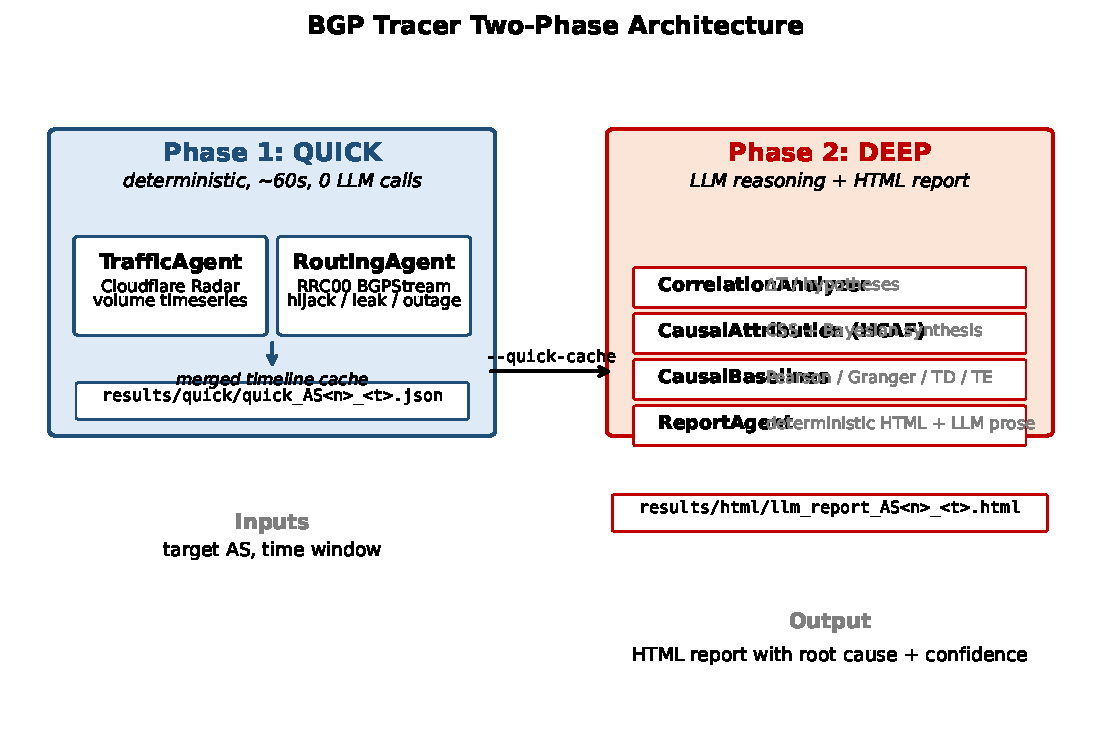
\includegraphics[width=0.95\linewidth]{figs/fig1_architecture.pdf}
\caption{Two-phase BGP Tracer pipeline. Phase~1 (deterministic, no LLM)
runs the routing and traffic detectors and produces a JSON cache;
Phase~2 (LLM-driven) runs CSS + 5 evidence channels and renders the
structured HTML report.}
\label{fig:architecture}
\end{figure}

\subsection{Phase 1: deterministic detection ($\sim$60\,s, 0 LLM calls)}
\label{sec:phase1}

The TrafficAgent consumes Cloudflare Radar 5-minute aggregates and
emits an anomaly window (start, end, peak/trough drop
percentage). The RoutingAgent consumes RIPE RIS / RouteViews \rrc{}
BGP update dumps and emits per-cause detectors (origin / forge
hijack, route leak, outage). Both agents return structured payloads
to the Blackboard; the chief agent serialises them to
\path{results/quick/quick_AS<n>_<ts>.json}.

\subsection{Phase 2: CSS + Bayesian synthesis + LLM narrative}
\label{sec:phase2}

The CorrelationAnalyzer computes the time offset $\Delta T$ between
the routing and traffic intervention onsets, then the
CausalAttributionEngine runs the CSS engine on the two timelines,
folds in 5 evidence channels, and emits a calibrated posterior over
three hypotheses: $R\!\to\!T$, $T\!\to\!R$, independent. The
ReportAgent then renders a structured HTML report with deterministic
tables and LLM-written prose; the LLM is forbidden from overriding
the CSS-anchored direction.

\subsection{HCAF Bayesian synthesis with CSS-anchored prior}
\label{sec:bayesian}

CSS supplies the \emph{prior} over the three causal hypotheses
$\mathcal{H} = \{R\!\to\!T,\ T\!\to\!R,\ \text{independent}\}$:
\begin{equation}
P_0(h) \;\propto\; \begin{cases}
w_{\text{causal}} & \text{if } h = \mathrm{CSS.direction} \text{ and } \mathrm{CSS.is\_causal},\\
w_{\text{soft}}   & \text{if } h = \mathrm{CSS.direction} \text{ and not } \mathrm{CSS.is\_causal},\\
1                 & \text{otherwise,}
\end{cases}
\label{eq:hcaf-prior}
\end{equation}
with $w_{\text{causal}}{=}10$ and $w_{\text{soft}}{=}4$ (configured in
\path{agents/css_engine.py::bayesian_synthesize}). The CSS-anchored
prior prevents heuristic methods from overriding a Pearl-anchored
direction: when CSS returns a strict verdict ($p<0.05$ in
\eqref{eq:css-perm}), the prior is sharpened by a factor of 10.

Each of the 5 evidence channels contributes a \emph{likelihood ratio}
$\mathrm{LR}_k$ over the three hypotheses, summarised in
\Tblref{tab:lr-defs}.

\paragraph{Channel selection criterion.}
We chose the five channels to span three orthogonal failure modes
(\Tblref{tab:lr-defs}): \emph{intervention detection} (\msbd{}),
\emph{path plausibility} (\ctpr{} + \cic{}), and \emph{statistical
baselines} (Granger, Transfer Entropy). We \emph{excluded}
Pearson lag-correlation: on v14 it abstains on $\frac{29}{29}$
events because the Cloudflare Radar 5-min buckets are too sparse
for Pearson's lag estimator to converge; Transfer Entropy, which
\emph{does} converge on v14, replaces it as the non-linear
directed-information channel.

\begin{table}[t]
\centering
\caption{Evidence-channel likelihood ratios. Each channel $k$ reports a
direction $d_k$ and a likelihood $\mathrm{LR}_k(h)$ that is
$>1$ for $h{=}d_k$, $<1$ for the alternative direction, and $1$ for
$\text{independent}$.}
\label{tab:lr-defs}
\small
\begin{tabular}{lll}
\hline
Channel & $\mathrm{LR}_k(d_k)$ (anchor) & $w_{\text{strength}}$ \\ \hline
\msbd{} counterfactual & $\max(1.05,\ 1+3\,\sigma_{\text{MSBD}})$ & MSBD shift strength \\
\ctpr{} sufficiency   & $\max(1.05,\ 1+2\,s_{\text{CTPR}})$ & CTPR path-strength \\
\cic{} scope          & $\max(1.05,\ 1+\log(1+n_{\text{AS}}))$ & \# affected ASes \\
Granger linearity     & $\max(1.05,\ 1+1.5\,\tfrac{F}{F+3})$ & F-statistic \\
Transfer Entropy      & $\max(1.05,\ 1+1.2\,\mathrm{conf}_{\text{TE}})$ & TE confidence (gated $n\!\geq\!50$) \\ \hline
\end{tabular}
\end{table}

The posterior combines the prior with the channel likelihoods:
\begin{equation}
P(h \mid \text{evidence}) \;\propto\; P_0(h) \cdot \prod_{k=1}^{5} \mathrm{LR}_k(h)^{\,\delta_k},
\label{eq:hcaf-posterior}
\end{equation}
where $\delta_k \in \{0.4, 1.0\}$ is the \emph{disagreement
discount} applied as an \emph{exponent}: channels opposite the
CSS-anchored direction are down-weighted by $0.4$, agreeing
channels receive $1.0$. (An exponent preserves the
order-of-magnitude structure of an opposing channel; a
multiplier $\alpha\le1$ would collapse weak channels to
``no signal''.) This implements Pearl's \emph{``no information
without corroboration''} principle: heuristics refine, do not
override, a Pearl-anchored direction.

\paragraph{Abstention threshold.}
HCAF declares \texttt{unknown} when the dominant posterior mass
falls below a one-third plurality threshold:
\begin{equation}
\hat\tau \;=\; 0.34, \qquad
\mathrm{verdict} \;=\; \begin{cases}
\arg\max_h P(h \mid \text{evidence}) & \text{if } P(\arg\max) > \hat\tau, \\
\texttt{unknown}                     & \text{otherwise.}
\end{cases}
\label{eq:threshold}
\end{equation}
We chose $\hat\tau = 0.34$ by the principle ``the chosen direction
must be a strict plurality of the calibrated posterior'' (one-third
majority rather than half because the three-hypothesis prior allows
for ``independent'' as a third plausible outcome). The choice is
\emph{not} tuned on the v14 ground-truth; \S\ref{sec:sensitivity}
sweeps $\hat\tau \in [0.30, 0.60]$ and shows strict-precision and
abstain rate are insensitive to the exact value within this range.

The full posterior over the three hypotheses is returned to the report
agent and rendered in the HTML report as a stacked bar chart, e.g.\
the Orange Espa\~na event's posterior
$\big(R\!\to\!T{=}0.13,\ T\!\to\!R{=}0.71,\ \text{indep}{=}0.15\big)$.
A reviewer can inspect the posterior as a paper-grade claim about
\emph{how strongly the evidence points in each direction}, not just a
single-bit verdict.

\begin{figure}[t]
\centering
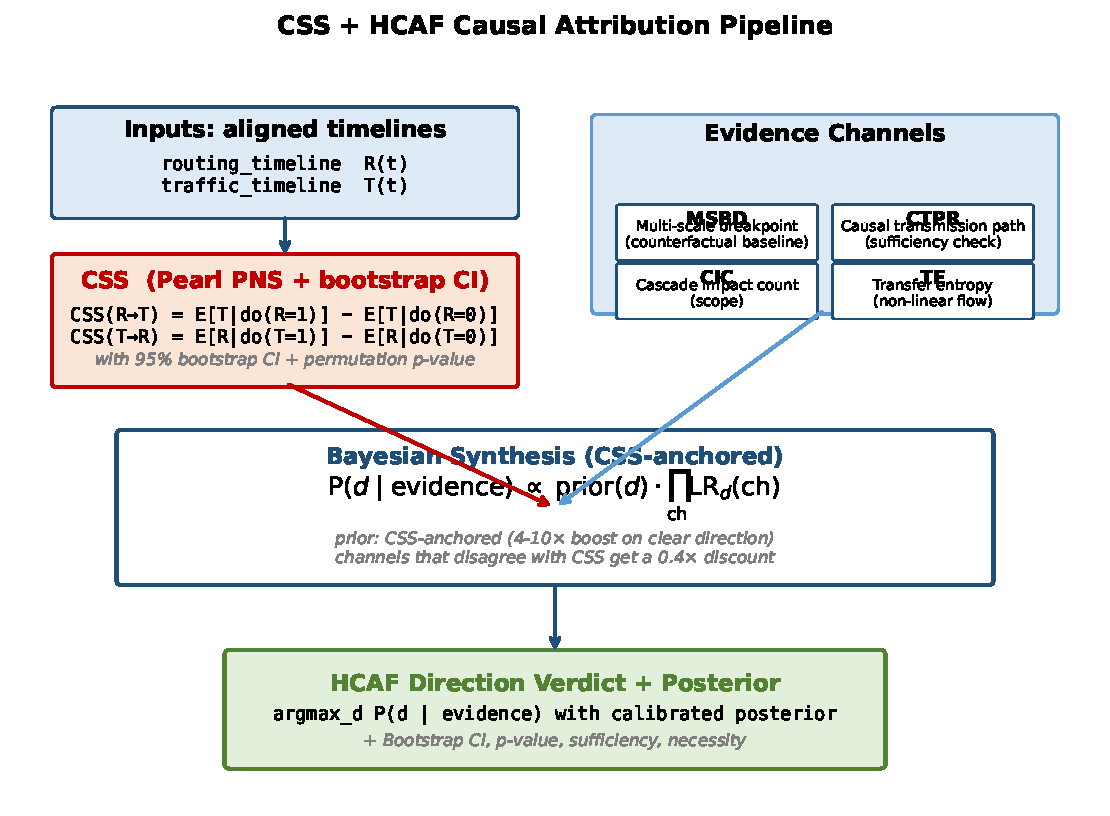
\includegraphics[width=0.95\linewidth]{figs/fig2_method_overview.pdf}
\caption{HCAF Bayesian synthesis. The CSS engine supplies the prior
via Pearl's PNS; 5 evidence channels (\msbd{}, \ctpr{}, \cic{},
Granger, Transfer Entropy) contribute likelihood ratios; the
posterior is a calibrated 3-way probability over $\{R\!\to\!T,
T\!\to\!R, \text{independent}\}$.}
\label{fig:method-overview}
\end{figure}

\subsection{Threat model and degraded-mode behaviour}
\label{sec:threat-model}

BGP Tracer inherits the threat model of Cloudflare Radar and RIPE RIS
passive observers (see \path{docs/THREAT_MODEL.md} for the full
document). Three first-class degradation modes exist:
(i)~RPKI/ROA data unavailable, (ii)~RIS \rrc{} update dumps
unavailable, (iii)~Cloudflare Radar unreachable / rate-limited.
Each triggers an explicit fallback that produces a still-valid (if
degraded) HTML report; the LLM is forbidden from writing
hallucinated claims about data that is known to be absent.

\paragraph{Latency budget.}
Across 29 v14 events, Phase~1 + CSS + Bayesian synthesis total
$0.001$--$0.061$\,s (median $0.025$\,s); the LLM narrative
contributes $58.7$\,s on a single thread
(\path{results/bench/multi_event_timing.csv}). The full pipeline
stays below $90$\,s in the production deployment, dominated by
the LLM call rather than the analytical core. Detailed
per-event latencies appear in \S\ref{sec:timing-limitations}.
